\documentclass[9pt,twocolumn,twoside,]{pnas-new}

% Use the lineno option to display guide line numbers if required.
% Note that the use of elements such as single-column equations
% may affect the guide line number alignment.


\usepackage[T1]{fontenc}
\usepackage[utf8]{inputenc}

% tightlist command for lists without linebreak
\providecommand{\tightlist}{%
  \setlength{\itemsep}{0pt}\setlength{\parskip}{0pt}}


% Pandoc citation processing
\newlength{\cslhangindent}
\setlength{\cslhangindent}{1.5em}
\newlength{\csllabelwidth}
\setlength{\csllabelwidth}{3em}
\newlength{\cslentryspacingunit} % times entry-spacing
\setlength{\cslentryspacingunit}{\parskip}
% for Pandoc 2.8 to 2.10.1
\newenvironment{cslreferences}%
  {}%
  {\par}
% For Pandoc 2.11+
\newenvironment{CSLReferences}[2] % #1 hanging-ident, #2 entry spacing
 {% don't indent paragraphs
  \setlength{\parindent}{0pt}
  % turn on hanging indent if param 1 is 1
  \ifodd #1
  \let\oldpar\par
  \def\par{\hangindent=\cslhangindent\oldpar}
  \fi
  % set entry spacing
  \setlength{\parskip}{#2\cslentryspacingunit}
 }%
 {}
\usepackage{calc}
\newcommand{\CSLBlock}[1]{#1\hfill\break}
\newcommand{\CSLLeftMargin}[1]{\parbox[t]{\csllabelwidth}{#1}}
\newcommand{\CSLRightInline}[1]{\parbox[t]{\linewidth - \csllabelwidth}{#1}\break}
\newcommand{\CSLIndent}[1]{\hspace{\cslhangindent}#1}


\templatetype{pnasresearcharticle}  % Choose template

\title{Abondance des espèces en fonction de la profondeur du site et le
moment de l'année}

\author[a,1,2]{Audrey-Ann Fortin, Amélie Garnier, Myriam Marentette}

  \affil[a]{Université de Sherbrooke}


% Please give the surname of the lead author for the running footer
\leadauthor{Anonymous}

% Please add here a significance statement to explain the relevance of your work
\significancestatement{}


\authorcontributions{}



\correspondingauthor{\textsuperscript{} }

% Keywords are not mandatory, but authors are strongly encouraged to provide them. If provided, please include two to five keywords, separated by the pipe symbol, e.g:
 \keywords{  Macroinvertébrés |  Qualité de
l'eau |  Benthos |  Inventaire |  Rivière  } 

\begin{abstract}

\end{abstract}

\dates{This manuscript was compiled on \today}
\doi{\url{www.pnas.org/cgi/doi/10.1073/pnas.XXXXXXXXXX}}

\begin{document}

% Optional adjustment to line up main text (after abstract) of first page with line numbers, when using both lineno and twocolumn options.
% You should only change this length when you've finalised the article contents.
\verticaladjustment{-2pt}



\maketitle
\thispagestyle{firststyle}
\ifthenelse{\boolean{shortarticle}}{\ifthenelse{\boolean{singlecolumn}}{\abscontentformatted}{\abscontent}}{}

% If your first paragraph (i.e. with the \dropcap) contains a list environment (quote, quotation, theorem, definition, enumerate, itemize...), the line after the list may have some extra indentation. If this is the case, add \parshape=0 to the end of the list environment.

\acknow{}

\hypertarget{ruxe9sumuxe9}{%
\section*{Résumé}\label{ruxe9sumuxe9}}
\addcontentsline{toc}{section}{Résumé}

Notre recherche se penche sur l'influence de la profondeur d'un site sur
les taxons retrouvés ainsi que la saison de l'année où l'échantillon est
prélevé. Cela a un impact important car on peut alors étudier l'impact
de d'autres facteurs, comme le réchauffement climatique, les nutriments
disponibles et la pollution, sur les populations des espèces puisqu'on
connait leur distribution dans le temps et l'espace.

\hypertarget{introduction}{%
\section*{Introduction}\label{introduction}}
\addcontentsline{toc}{section}{Introduction}

Les communautés de macroinvertébrés peuvent être utilisées comme
indicateur permettant permet d'avoir une idée de la santé de
l'écosystème aquatique étudié. Les macroinvertébrés sont un échelon
essentiel du réseau trophique des rivières, nourrissant poissons,
oiseaux et d'amphibiens. Leur abondance peut donc donner une idée de
l'état du plan d'eau. (1) Avec les changements climatiques et la
pollution, l'environnement change, ce qui peut bouleverser l'écosystème
aquatique entier. La densité de microinvertébrés peut varier entres
autres en fonction de la quantité de nutriments disponibles, du type de
nutriments et du taux d'oxygène dans l'eau. L'étude des macroinvertéprés
peut donc aussi être un indicateur d'eutrophisation. (2) Notre étude
vise à déterminer si la profondeur d'un site d'observation a un imact
sur le type d'organisme qu'on y retrouve. Nous voulons aussi explorer la
variation de la présence des différents taxons à l'étude selon le temps
de l'année. Ces connaissance pourront servir à d'autres études visant à
des projections dans les changements de réseau trophiques et prévoir
quelles espèces seront présentes sur un nouveau site d'étude.

\hypertarget{muxe9thode}{%
\section*{Méthode}\label{muxe9thode}}
\addcontentsline{toc}{section}{Méthode}

Les inventaires du benthos sont réalisés à l'aide d'un filet à mailles
fines (D-net) qui est traîné sur le fond de la rivière à trois reprises.
L'effort d'échantillonnage est de 3m². Les échantillons sont ensuite
ramenés en laboratoire et étalés sur des plateaux de tri « Bogorov » où
les espèces sont identifiées et dénombrées. Seule une portion (fraction)
de l'échantillon est analysée. L'abondance des espèces est calculée en
fonction de la quantité d'individus trouvés dans l'échantillon et de la
fraction analysée. (3) Pour le traitement des données, nous avons
procédé à un nettoyage de toutes les données recueillies, s'assurant
qu'elles étaient exemptes d'erreurs. Nous les avons ensuite rassembée
dans une seule grande base de donnée, dont nous nous sommes servi pour
analyser la distribution des espèces grâce à différents types de
graphiques.

\hypertarget{ruxe9sultats}{%
\section*{Résultats}\label{ruxe9sultats}}
\addcontentsline{toc}{section}{Résultats}

\begin{figure}
\centering
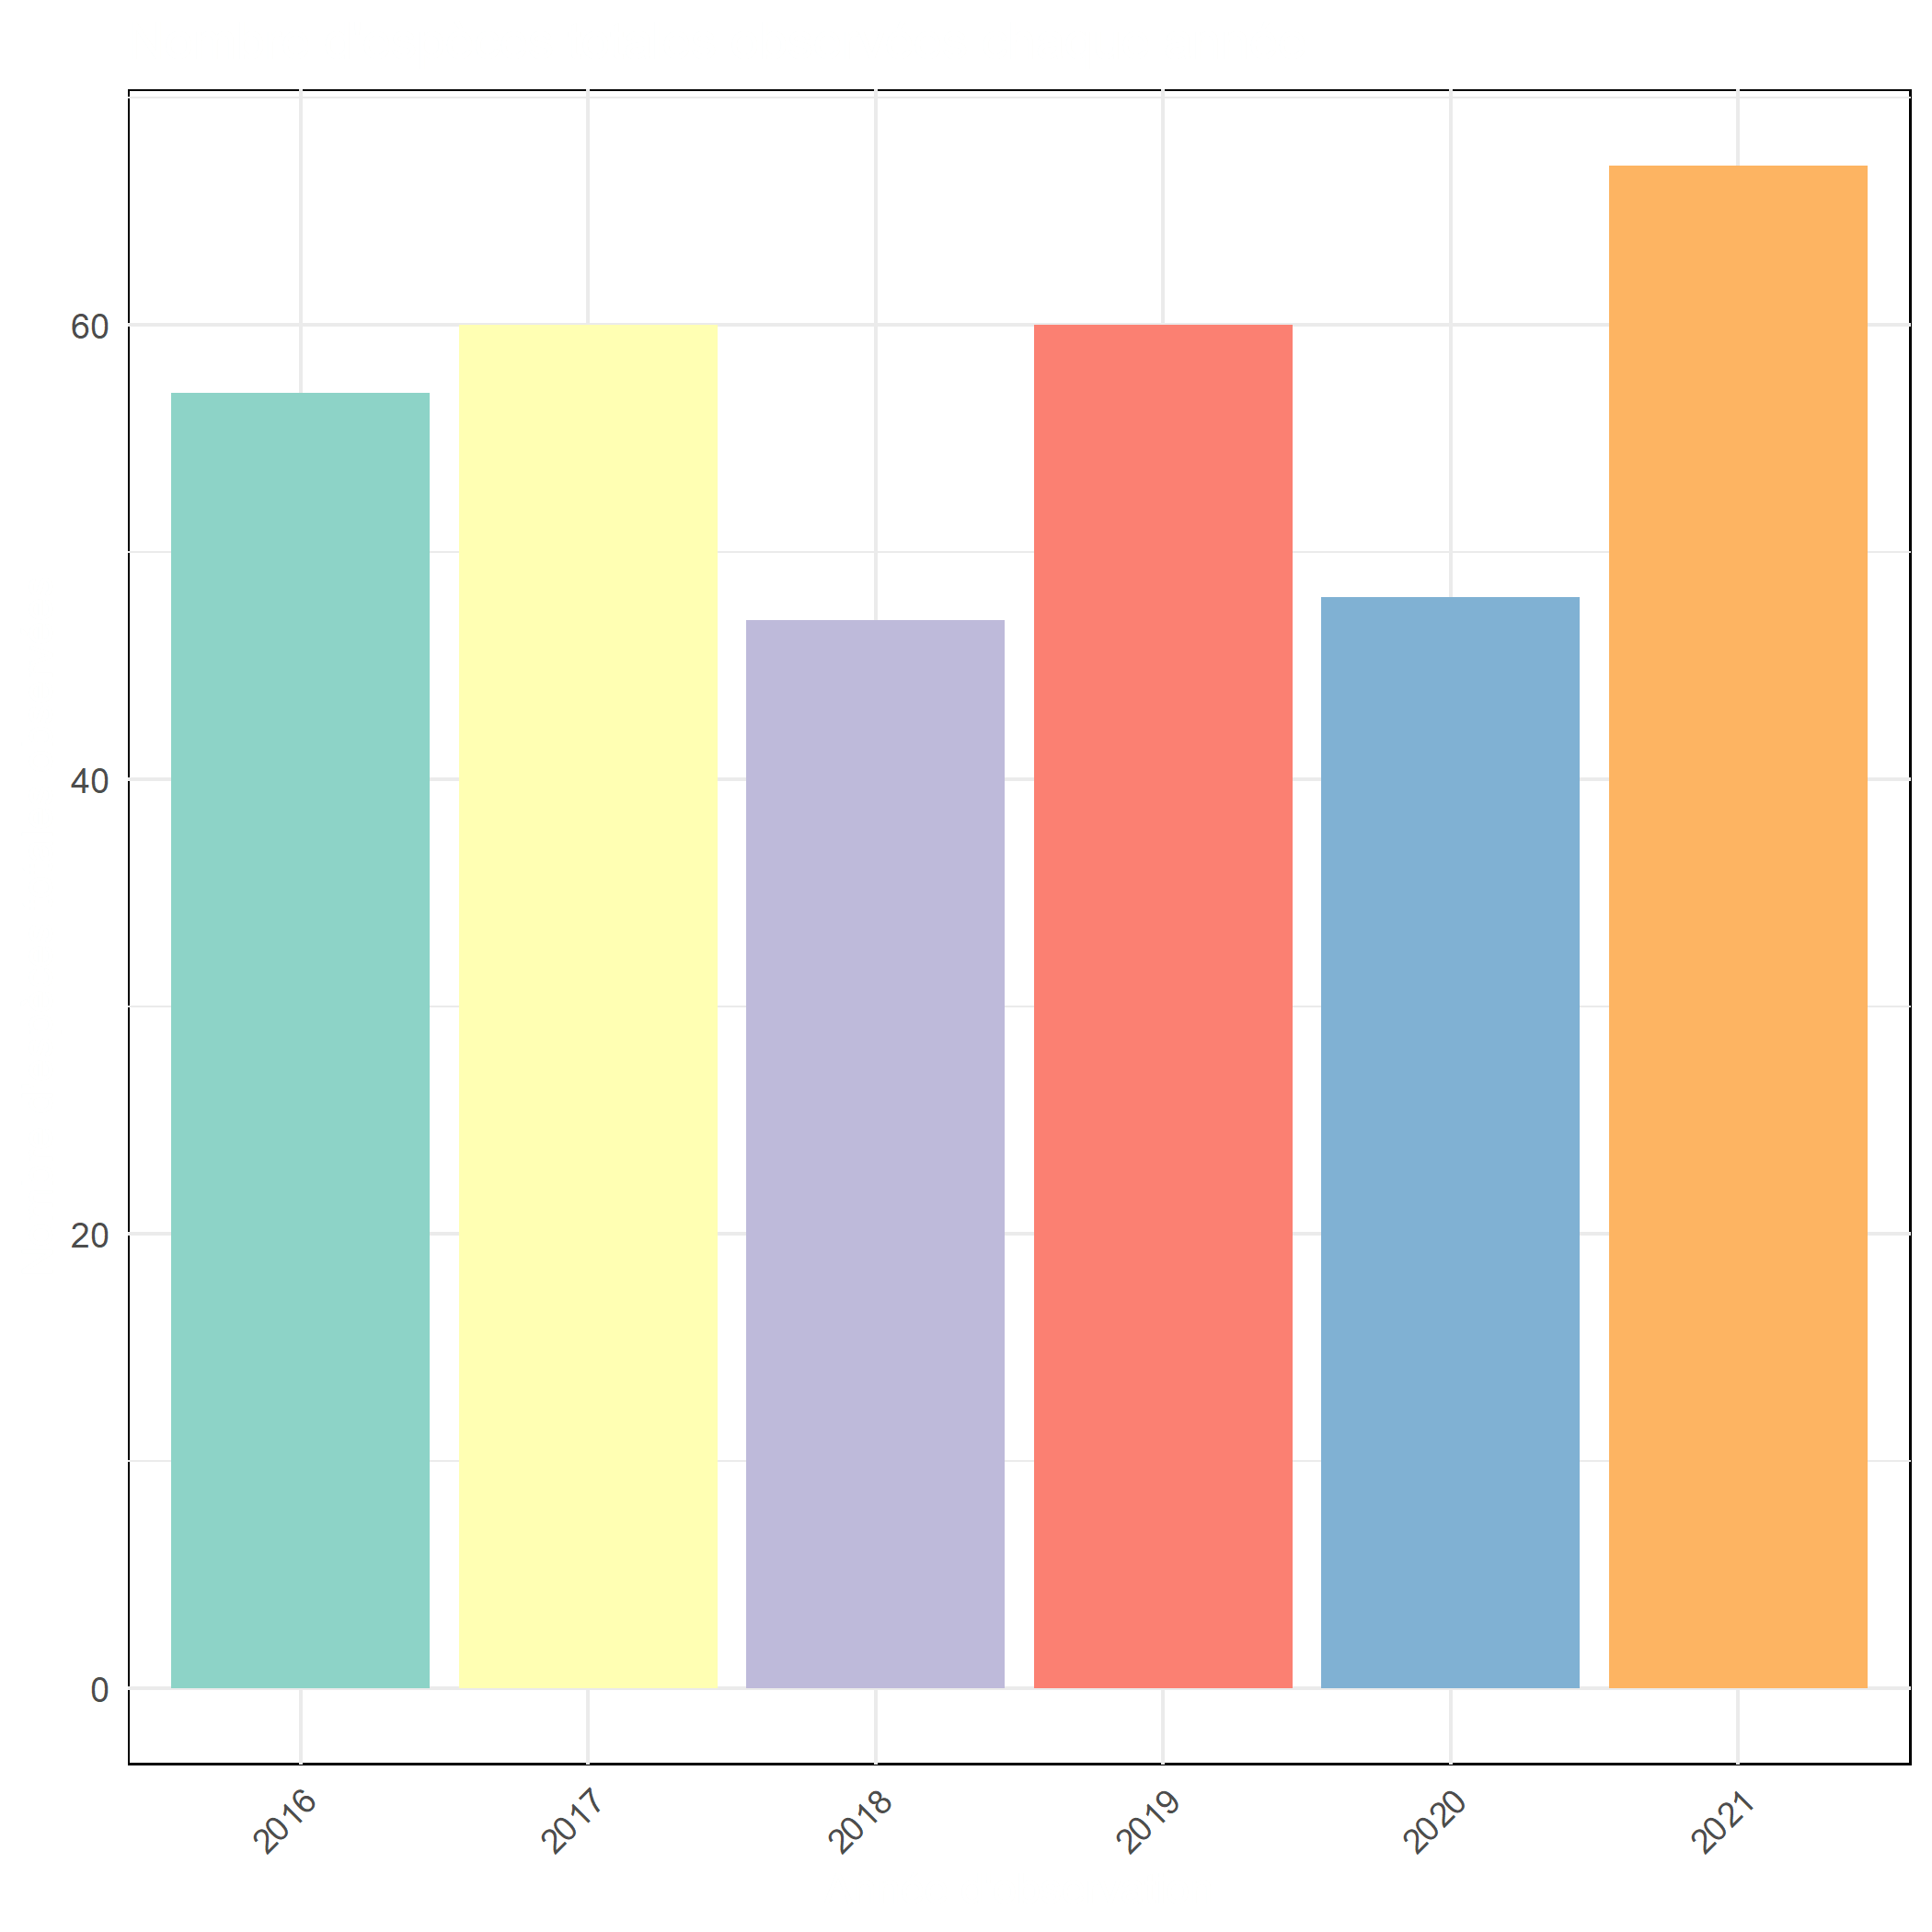
\includegraphics[width=0.5\textwidth,height=0.4\textheight]{"/Users/sylvie/Desktop/BIO500/Projet-Benthos-main/Projet-Benthos/RAPPORT/figures/figure_un.png"}
\caption{figure1. \label{fig1}}
\end{figure}

La première figure montre l'a courbe'histogramme du nombre d'espèces
observées par années. On remarque que malgré une certaine variation, le
nombre d'espèce semble se maintenir deuis 2016, ce qui est bon signe. Si
les macroinvertébrés sont toujours présents, c'est que le réseau
trophique n'est pas trop touché par les changements environnementaux
pour le moment.

\begin{figure}
\centering
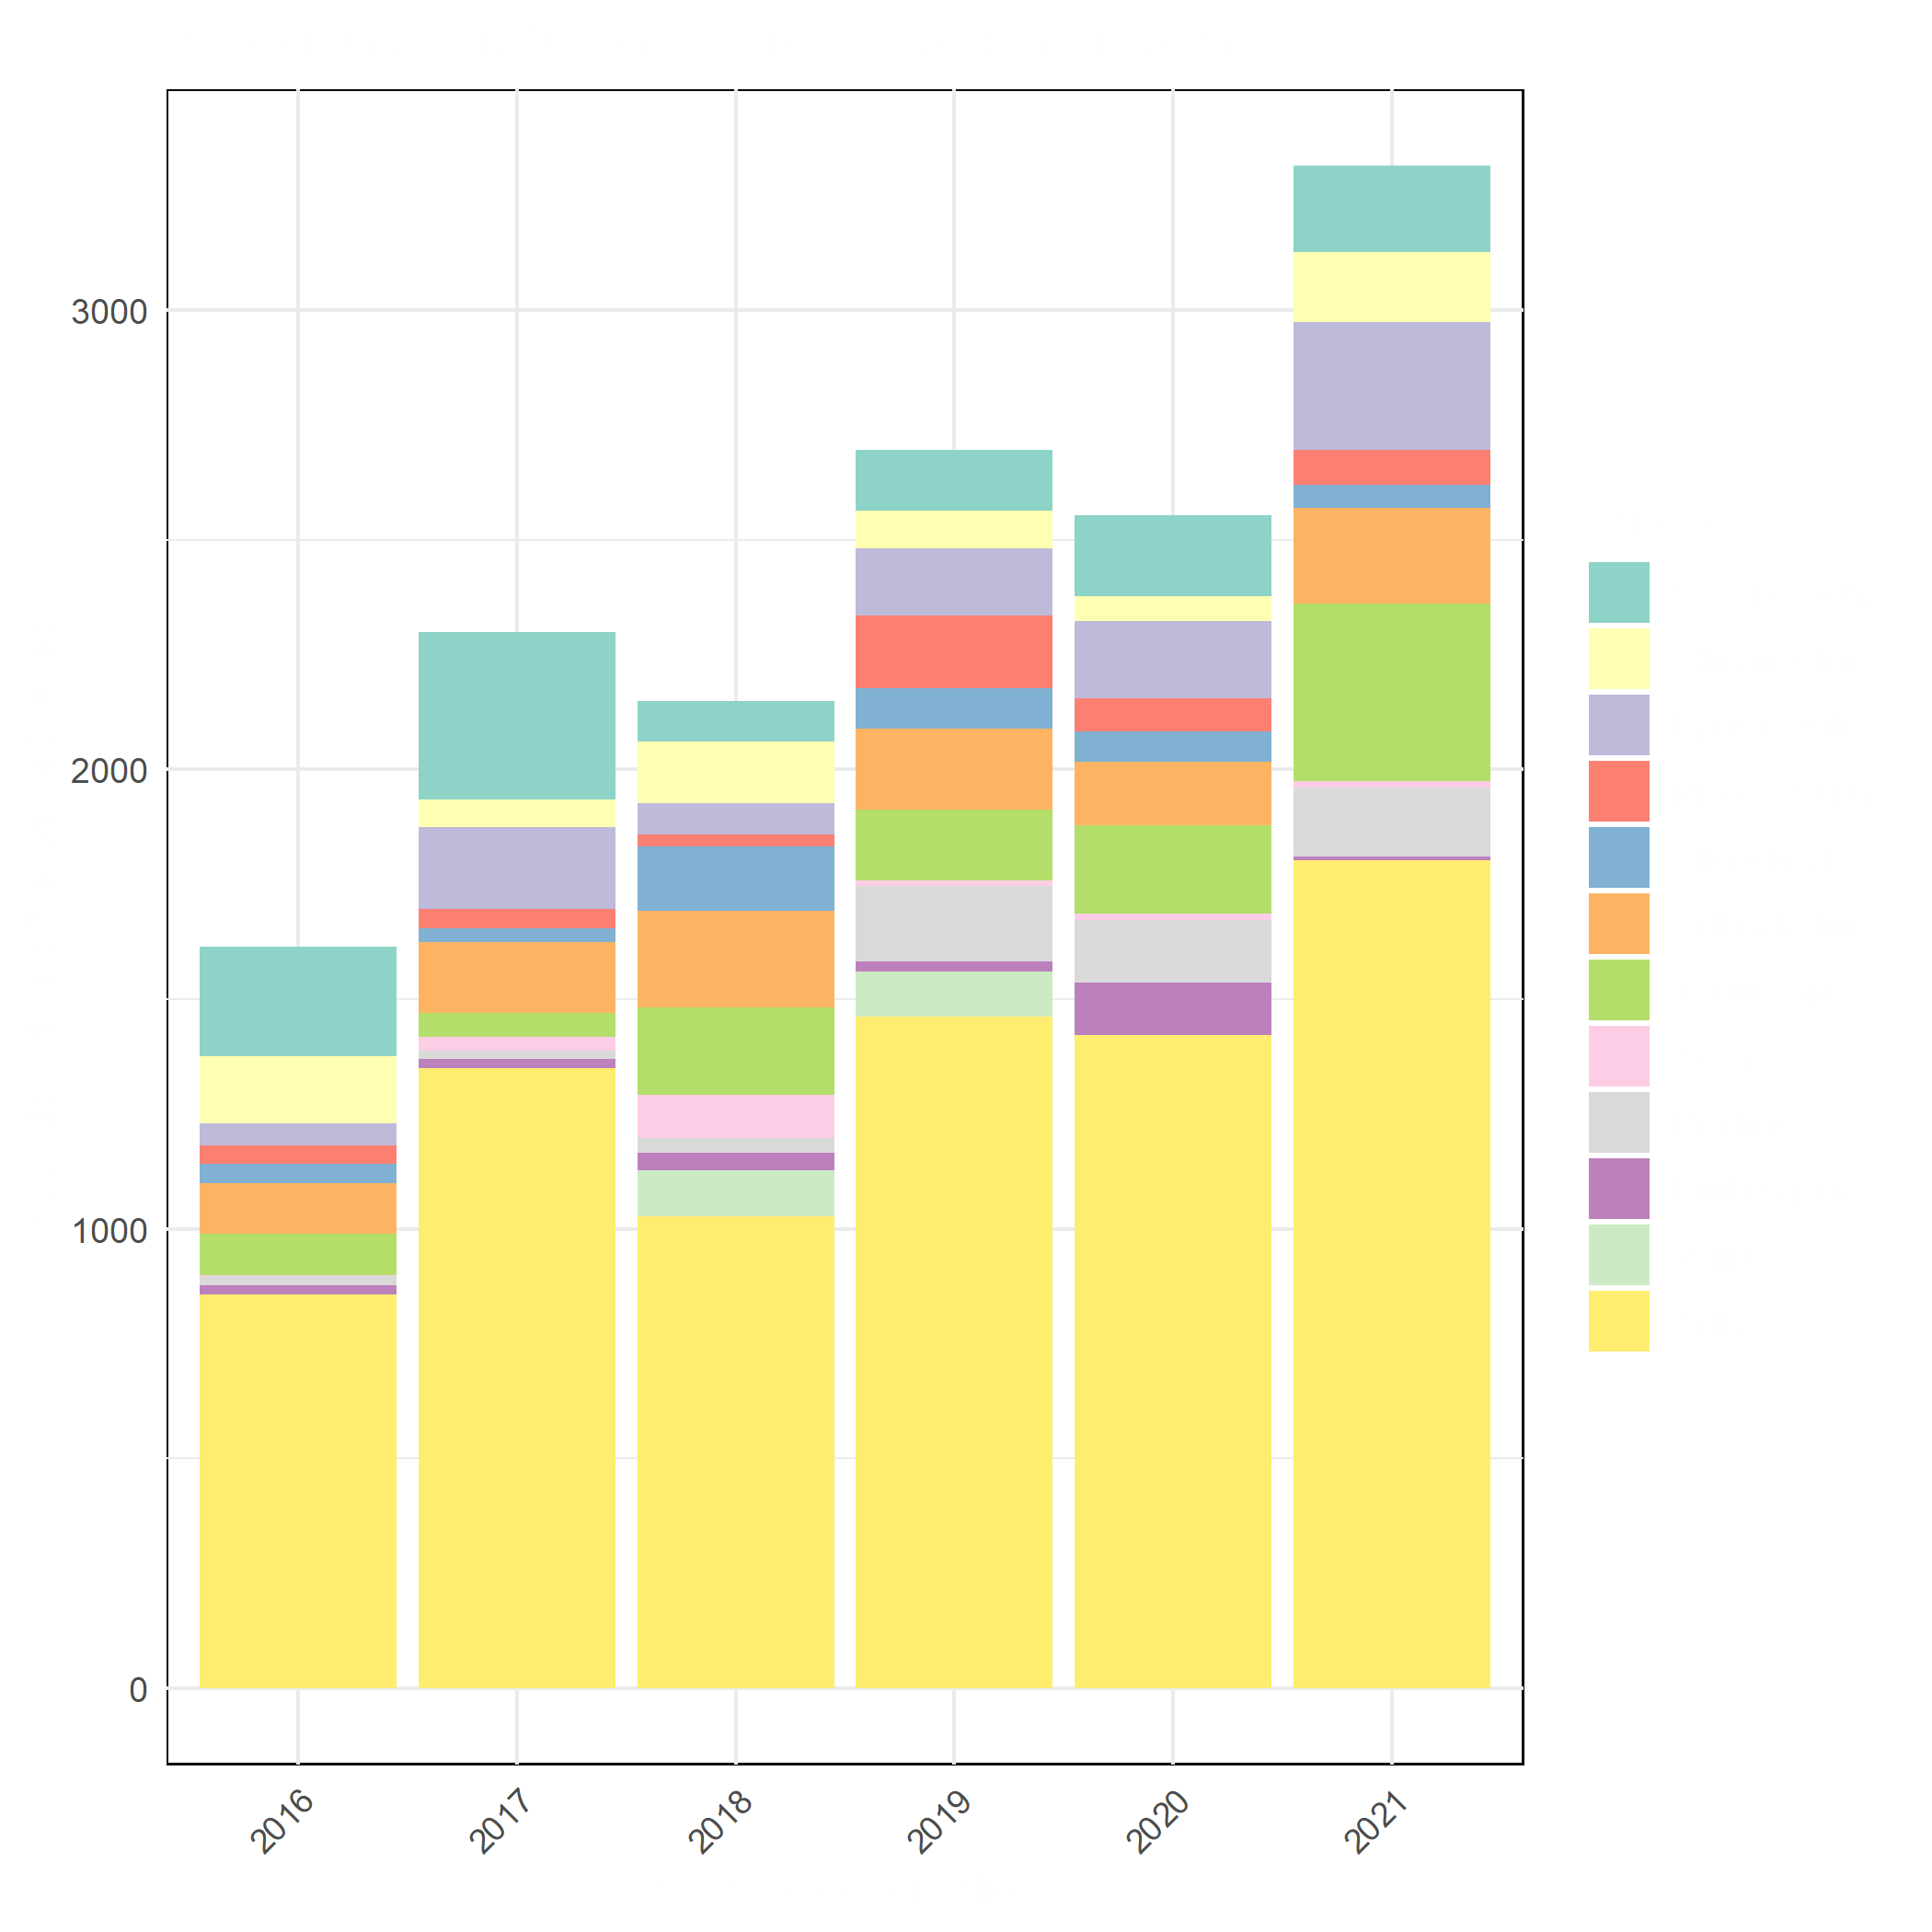
\includegraphics[width=0.5\textwidth,height=0.4\textheight]{"/Users/sylvie/Desktop/BIO500/Projet-Benthos-main/Projet-Benthos/RAPPORT/figures/figure_deux.png"}
\caption{figure1. \label{fig1}}
\end{figure}

La seconde figure montre l'abondance relative par espèce selon l'année
d'observation. On peut donc voir quelles sont les espèces les plus
présentes chaque année et la proportion qu'elles occupent parmis la
biodiversité totale des macrocrustacés. On observe au fil des années une
augmentation de la population de Tanytarsini, et une diminution de
Rhithrogena. Cela peut être dû aux changements environnementaux qui
peuvent avantager certains organismes et nuire à d'autres.

\begin{figure}
\centering
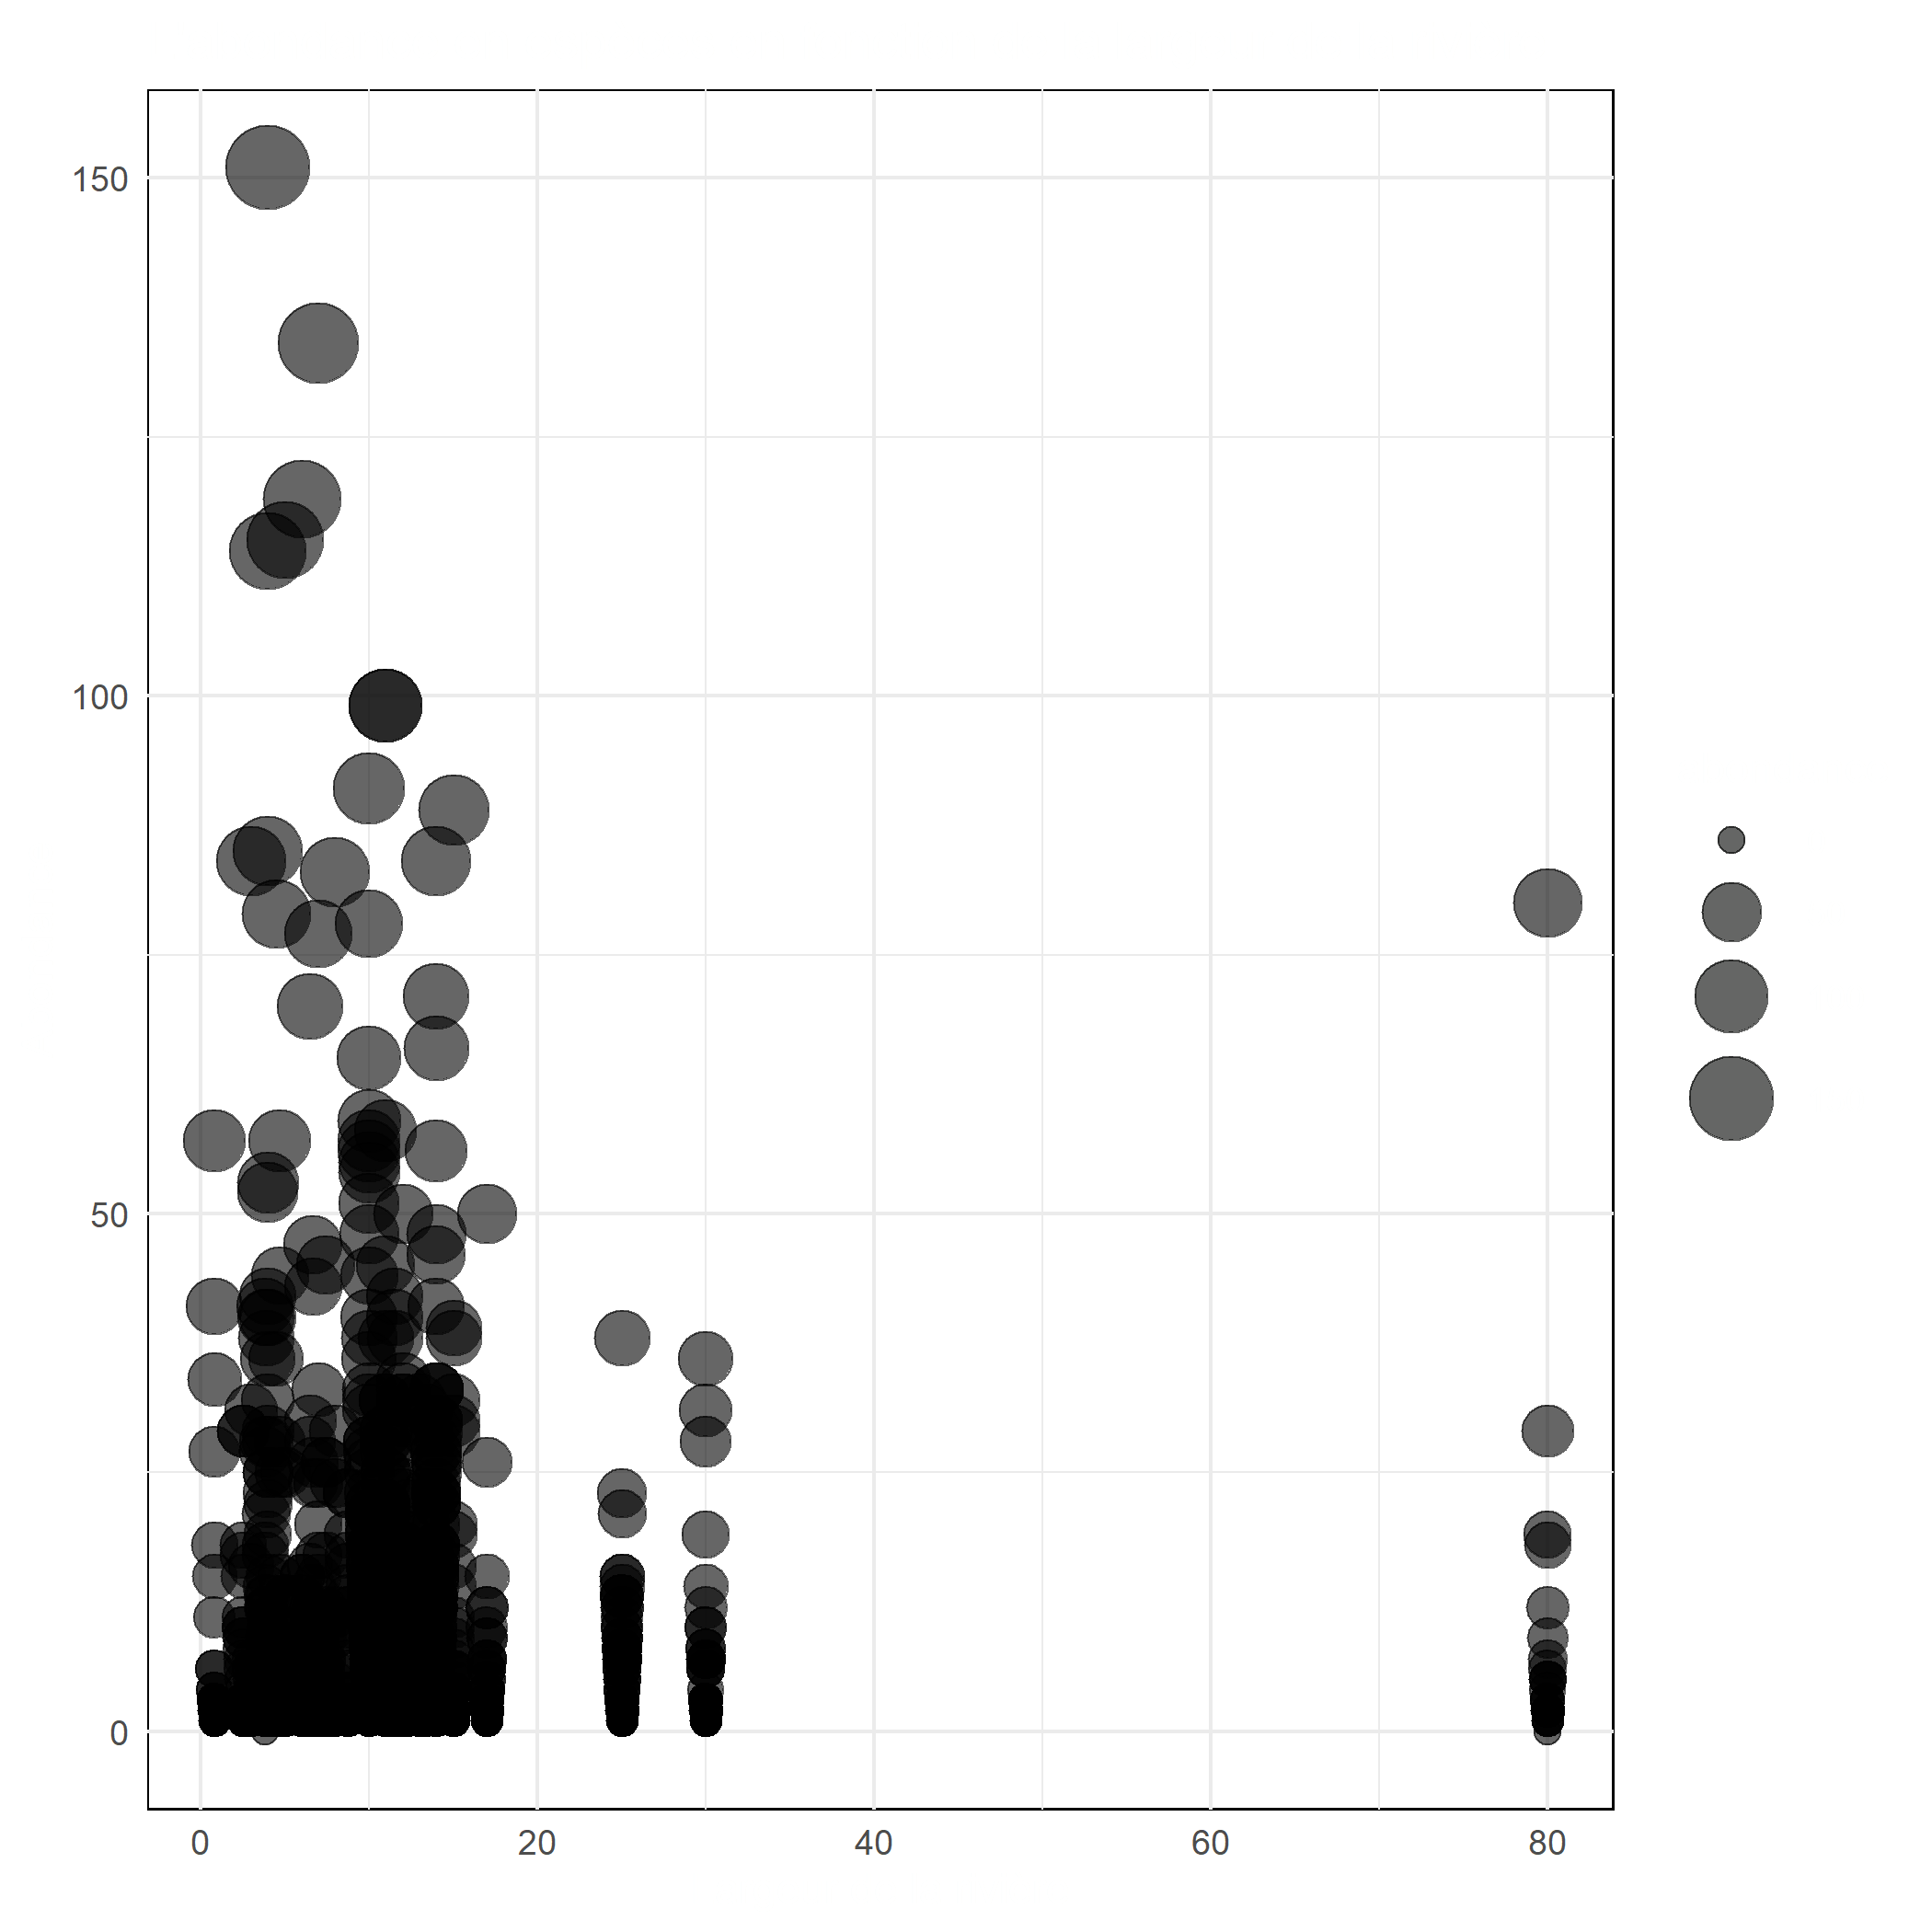
\includegraphics[width=0.5\textwidth,height=0.4\textheight]{"/Users/sylvie/Desktop/BIO500/Projet-Benthos-main/Projet-Benthos/RAPPORT/figures/figure_trois.png"}
\caption{figure1. \label{fig1}}
\end{figure}

La troisième figure montre l'abondance d'espèces selon la largeur de la
rivière. On obserbe que plus la rivière est étroite, plus nombreuses
sont les espèces observées. Il semble y avoir un reguain dans la
quantité d'espèces quand la rivière a une largeur de 80m. Il se peut
toutefois que cela soit dû à une erreur.

\begin{figure}
\centering
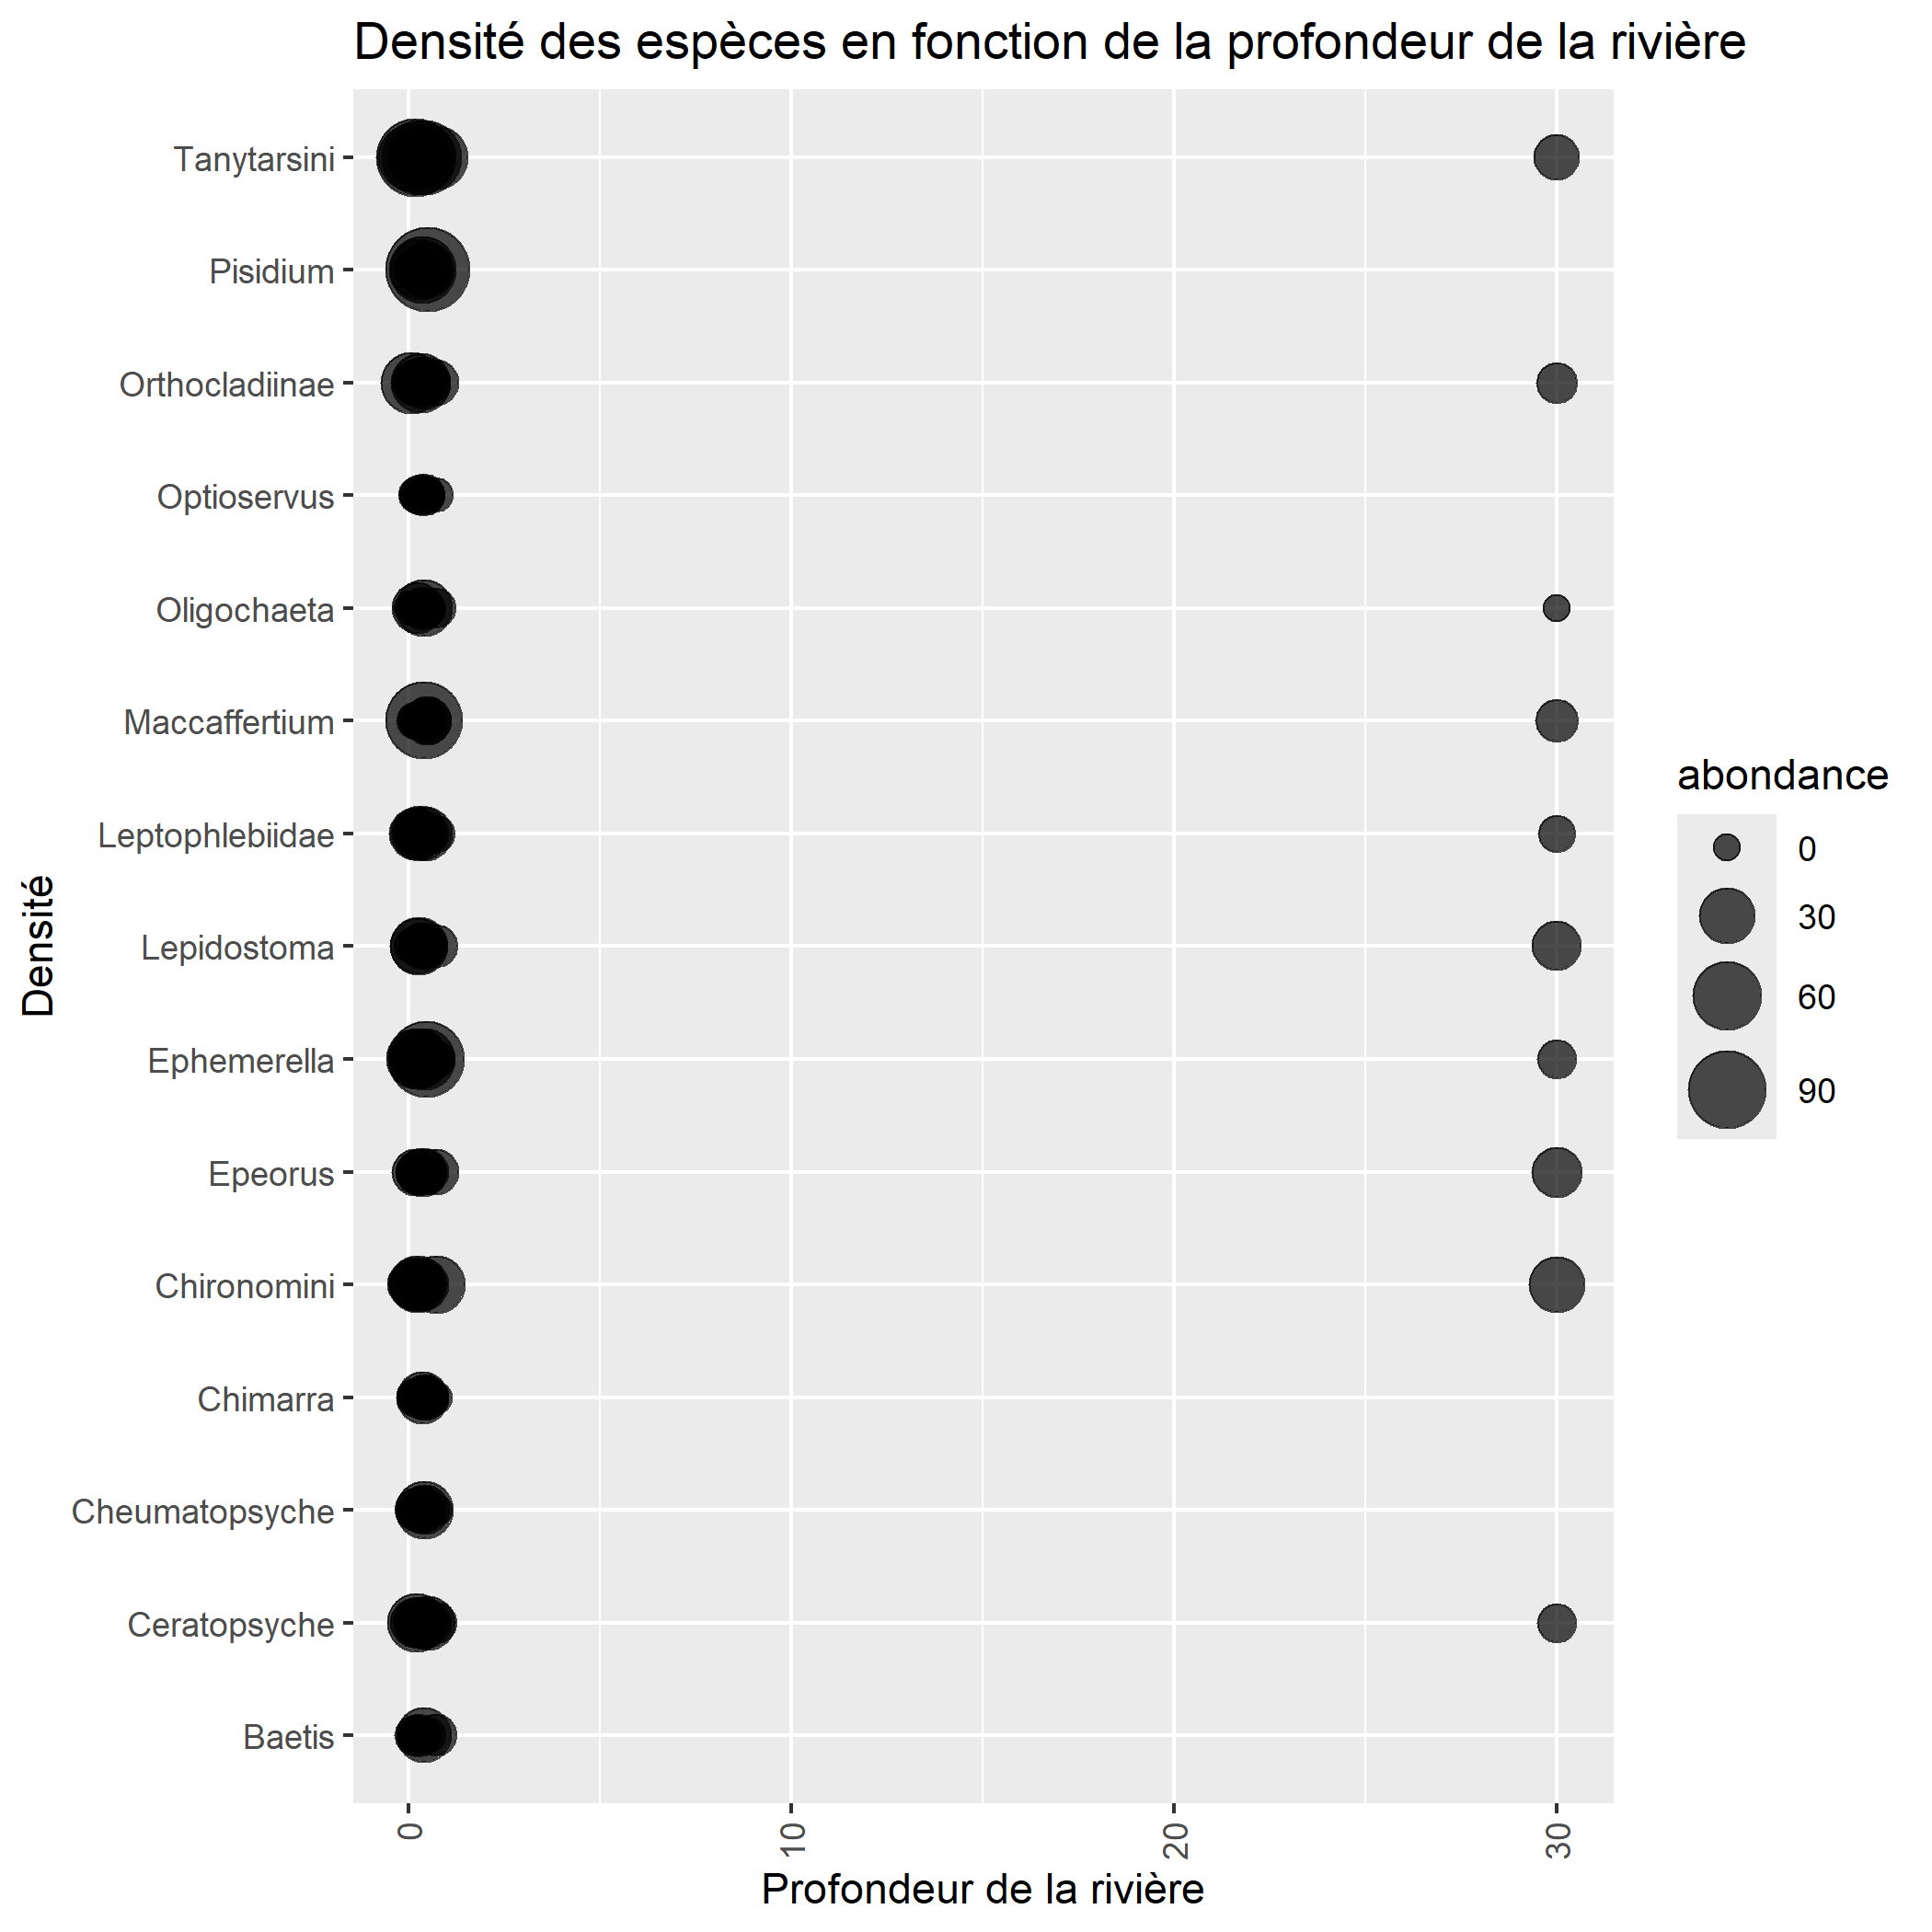
\includegraphics[width=0.5\textwidth,height=0.4\textheight]{"/Users/sylvie/Desktop/BIO500/Projet-Benthos-main/Projet-Benthos/RAPPORT/figures/figure_quatre.png"}
\caption{figure1. \label{fig1}}
\end{figure}

La dernière figulre, la quatrième, présente la densité des populations
de chaque espèces selon cette foi la profondeur de la rivière. Encore
une fois, moins elle est profonce, plus nombreux sont les organismes. On
observe ici aussi un deuxième pic, à 30, et cela peut être dû à la même
erreur.

\showmatmethods
\showacknow
\pnasbreak

\hypertarget{refs}{}
\begin{CSLReferences}{0}{0}
\leavevmode\vadjust pre{\hypertarget{ref-guide2013}{}}%
\CSLLeftMargin{1. }%
\CSLRightInline{Moisan J, Pelletier L (2013) Guide de surveillance
biologique basée sur les macroinvertebres benthiques d'eau douce du
québec. \emph{Centre d'information du ministère du Développement
durable, de l'Environnement, de la Faune et des Parcs}:89.}

\leavevmode\vadjust pre{\hypertarget{ref-ponds2017}{}}%
\CSLLeftMargin{2. }%
\CSLRightInline{Moss B (2017) \emph{Ponds and small lakes,
microorganisms and freshwater ecology} (Pelagic publiching).}

\leavevmode\vadjust pre{\hypertarget{ref-protocole2011}{}}%
\CSLLeftMargin{3. }%
\CSLRightInline{Moisan J, Pelletier L (2011) Protocole d'échantillonnage
des macroinvertébrés benthiques d'eau douce du québec. \emph{Centre
d'information du ministère du Développement durable, de l'Environnement,
de la Faune et des Parcs}:41.}

\end{CSLReferences}



% Bibliography
% \bibliography{pnas-sample}

\end{document}
